\documentclass[10pt, journal]{IEEEtran} % TODO find out what is journal
\renewcommand{\familydefault}{phv}
\renewcommand{\rmdefault}{phv} % Arial
\renewcommand{\sfdefault}{phv} % Arial
\usepackage[a4paper, margin=1in]{geometry} % paper size and margin
\usepackage{microtype} % prevent word breaks
\usepackage{cite} % TODO learn how to use
\usepackage{tikz} % for plantuml exports
\usepackage{graphicx} % TODO what does this do?
\usepackage{float} % force images into text
\usepackage{caption} % TODO what does this do?

\usepackage{pgffor} % for sourcecode
\usepackage{listings} % for sourcecode
\usepackage{color} % for sourcecode
\usepackage{url} % to show URLs

\graphicspath{ {./images/} } % path where images are stored

% TODO Florida Atlantic University
\title{
    Use of IoT Sensor Networks in the Home \\
    }

\author{
    Abir Faisal, Paris Isley, Tutku Gizem \\
    \small Group: UG18-4164 \\
    \small CNT4164 - Intro to IOT and Sensor Networks - Final Project \\
    \small Prof. Mohammad Ilyas \\
    \smallskip
    \small Project Repository: \url{https://github.com/AbirFaisal/CNT4164_GroupProject}
    % \small Department of Electrical Engineering and Computer Science, Florida Atlantic University
    }


\markboth{Department of Electrical Engineering and Computer Science, Florida Atlantic University, Fall 2025}{} %{left head}{right head}

\begin{document}

\twocolumn[ % force abstract to use two columns.

% prevent page break
\begin{@twocolumnfalse}
    \maketitle
\end{@twocolumnfalse}


\begin{abstract}
    A brief summary of the entire paper, including the research question, methodology, key findings, and conclusions. 
\end{abstract}

\begin{IEEEkeywords}
    Sensor Networks, IoT, Internet of Things, Smart Homes
\end{IEEEkeywords}

\noindent\rule{\textwidth}{1pt}
% \bigskip
\smallskip
]

\section{Introduction}

The idea of the smart home has been around for a long time.
IoT devices enable the smart devices to be networked.
The use of these devices can provide users with several advantages,
such as increased comfort, increased safety, improved home management and maintainance,
energy savings, automation and convenience in general.

Furthermore, sensor networks augment the use of IoT devices by collecting data around the home.
Unlike centralized sensing, a network of sensors can provice a more granular understanding of the enviornment.
These sensors can be placed throughout the home, and connect using existing network infrastructure.

In this report we show the use of a sensor network that could be used for climate control.

\section{Project Description}

We are using an RP2040W as an IoT device, this will contain a web interface and it will
query nodes on the sensor network.
We did not have adequete time to implement this in hardware,
it is being mentioned for the purpose of explaining the concept.

We're using an ESP01 devices as a nodes for the sensor network.
It will be paired with an AHT20 temperature and humidity sensor, 
which will be connected to the ESP01 over i2c.

The combination of the IoT device and the sensor network will create a smart system, specifically a smart thermostat.
In this implimentation, 
the IoT device also serves as the smart system because it would have direct control of the air conditioner.

\subsection{Sensor}

An image of the sensor node can be seen in [Figure \ref{fig:sensor}].
The buttons are only for debugging purposes such as resetting the controller 
and putting it into programming mode to flash the firmware.
They are not used for any other function.

Setting up the device on the network is simple.
The device presents a WiFi access point that you can connect to using your phone or computer.
After you connect, a captive portal is presented where you can enter the necessarry credentials 
such as the WiFi SSID and the password to connect the sensor to the network.
After this the device connects to the specified network,
and presents a server that returns a JSON that contains the readings for the onboard sensors.
If the network configureation is changed, or the device is unable to find or connnect to the configured network,
the device presents an access point again and the user can repeat this process.

\begin{figure}[h]
    \centering
    \includegraphics[width=0.4\textwidth]{images/sensor.png}
    \caption{ESP01 + AHT20 Sensor}
    \label{fig:sensor}
\end{figure}



\section{Results}

The sensor responds with a JSON formatted string when sent an HTTP request to it's IP Address.
[Figure \ref{fig:sensor_response}]

Here is an sample:

\lstinline[basicstyle=\footnotesize]|{"id": 1, "temperature": 25.347, "humidity": 35.634}|

The temperature is reported in celsius, and the humidity is reported in percent relative humidity.

\begin{figure}[htpb]
    \centering
    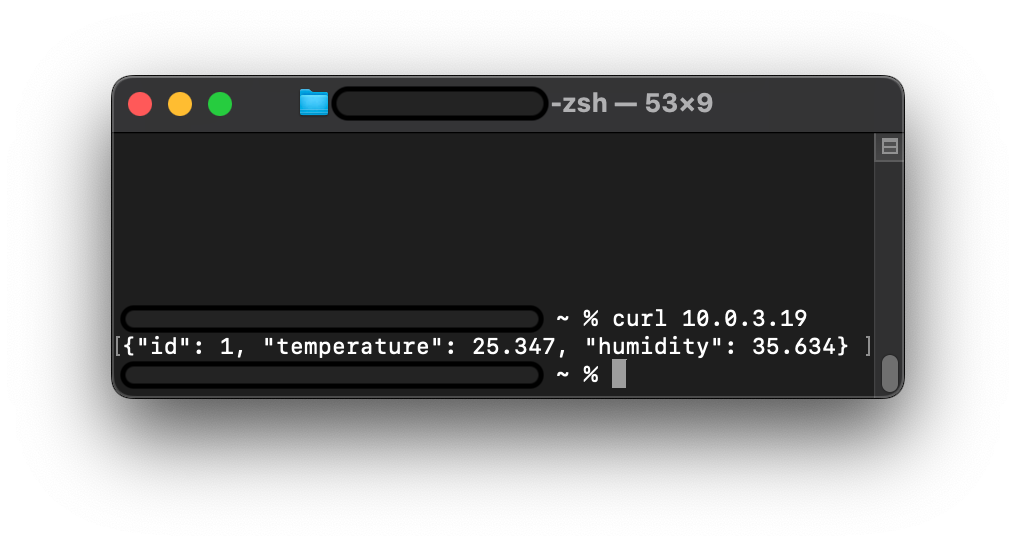
\includegraphics[width=0.4\textwidth]{images/sensor_response.png}
    \caption{Response from sensor}
    \label{fig:sensor_response}
\end{figure}


\section*{IoT Devices in Home Sensor Networks}

There are many areas where a sensors can be used in the home.
Here is a list of examples:

\begin{itemize}[]  % Customized list with more spacing
    \item{\textbf{Security and Surveillance}}
        \begin{itemize}
            \item Smart cameras
            \item Motion detectors
            \item Window/door sensors
            \item Security alarm systems
            \item Personnel Detection
            \item Intrusion Detection
        \end{itemize}

    \item{\textbf{Climate Control}}
        \begin{itemize}
            \item Smart thermostats
            \item Air quality sensors (e.g., particulate matter, CO2)
            \item Humidity sensors
            \item Temperature sensors
            \item Smart air purifiers
        \end{itemize}

    \item{\textbf{Lighting}}
        \begin{itemize}
            \item Smart bulbs
            \item Smart switches and outlets
            \item Motion-activated lighting
            \item Color-changing LED strips
            \item Outdoor lights with timers/sensors
        \end{itemize}

    \item{\textbf{Energy and Resource Monitoring}}
        \begin{itemize}
            \item Smart plugs
            \item Energy monitoring systems
            \item Smart meters for electricity, gas, or water
            \item Power strips with energy tracking
            \item Grid Power
            \item Solar Panels
        \end{itemize}

    \item{\textbf{Audio and Video}}
        \begin{itemize}
            \item Smart speakers (e.g., Amazon Echo, Google Nest)
            \item Soundbars with smart features
            \item Wi-Fi enabled headphones
            \item Streaming devices (e.g., Roku, Apple TV)
            \item IP intercom systems
        \end{itemize}

    \item{\textbf{Cooking and Appliance Control}}
        \begin{itemize}
            \item Smart ovens/ranges
            \item Coffee makers
            \item Connected refrigerators with inventory management
            \item Dishwashers with smart scheduling
            \item Microwave ovens
        \end{itemize}

    \item{\textbf{Entertainment and Gaming}}
        \begin{itemize}
            \item Smart TVs with built-in apps
            \item Video game consoles (e.g., Xbox One, PlayStation 4)
            \item VR headsets with home tracking sensors
            \item Home theater systems with smart features
        \end{itemize}

    \item{\textbf{Health and Wellness}}
        \begin{itemize}
            \item Smartwatches/fitness bands (e.g., Apple Watch, Fitbit)
            \item Blood pressure monitors
            \item Weight scales with data tracking
            \item Sleep monitoring devices
            \item Smart water bottles with usage tracking
        \end{itemize}

    \item{\textbf{Home Automation}}
        \begin{itemize}
            \item Smart hubs (e.g., Amazon Alexa, Google Home)
            \item Zigbee or Z-Wave compatible devices
            \item Automated curtains and blinds
            \item Smart locks with keyless entry
            \item Connected garage door openers
        \end{itemize}

    \item{\textbf{Water Management}}
        \begin{itemize}
            \item Water leak detectors
            \item Smart sprinklers with soil moisture sensors
            \item Toilet overflow sensors
            \item Smart water heaters
        \end{itemize}

    \item{\textbf{Miscellaneous Smart Devices}}
        \begin{itemize}
            \item Smart mirrors with calendar/weather displays
            \item Connected waste bins with fill level monitoring
            \item Smart key fobs for location tracking
            \item Plant monitors for soil moisture and light levels
            \item Smart pet feeders
        \end{itemize}

    \item{\textbf{Tangenial Technologies}}
        \begin{itemize}
            \item Smart Cars
            \item Healthcare
        \end{itemize}

\end{itemize}



% TODO REMOVE BEFORE SUBMISSION:

% Who, what, when, where, how, and whys

% Each section to have:
% - Usage, how are IoT technologies useful in this context?
% - Market, who would use these devices?
% - Security, how are the devices secured?
% - Topology, how do the devices communicate?
% - Sensors, what sensors could the devices have?
% - Measurement, how or what do the sensors measure?
% - Power, How are the devices powered?


% TODO REMOVE BEFORE SUBMISSION

\section{Internet of Things, Sensor Networks, and Smart Systems}

The IoT device in this use case serves two main responsabilties 
querying the sensors on the network, and providing a web interface.

The web interface should present a dashboard to the user where they can
monitor the temperature and set preferences.


\subsection{Smart System}

A smart thermostat would take measurements from the sensor network to make decisions.

Using the average of the sensors, biased by the hightest or lowest reading,
the thermostat would know how to maintain the temperature of the room.


Assume $S$ is a set of readings from the sensor network:

$S = \{sensor_1, sensor_2, sensor_3, ...sensor_n\}$

\bigskip

If the thermostat is set to maintain coolness,
then the the highest reading would be used as the bias:

\[
T_c = \frac{1}{n+1}\left[ \max_{s \in S} + \sum_{s \in S}{s} \right]
\]

\smallskip

If the thermostat is set to heat,
then the lowest temperature reading would be used as the bias:

\[
T_c = \frac{1}{n+1}\left[ \min_{s \in S} + \sum_{s \in S}{s} \right]
\]

Where $T_c$ is the computed temperature.

\bigskip


It is possible to create a smart system that automatically heats and cools as needed,
but this can result in a control loop that oscillates if not done correctly.
This is why thermostats generally do not have this functionality.
A control loop such as PID can manage a system like this,
however the engineering expense for such a system would far exceed the benefits 
outside of a controlled environment such as a labratory.
A common change such as new furniture or home improvement
can require recalibation of the PID parameters.

A simple solution for this can be the use of threshold values.
This assumes that the average daily temperature fluxuation is known.
If the temperature is within the specified range, nothing is done,

For example a target temperature of 75 is set, with a range of 68-78.
If the temperature rises above 78, the system cools to 75,
if the temperature drops below 68, the system heats to 75.

\[
T_c = \frac{1}{n}\sum_{s \in S}{s}
\]

$heat = T_c < T_l$

$cool = T_c > T_u$

$action = argmax(heat, cool)$

\smallskip

Where $T_l$ is the lower bound, and $T_u$ is the upper bound.

\bigskip

As long as the average daily temperature fluxuation is within the bounds,
this system should not oscillate.

Furthermore such a system would be simple enough for an end user to configure themselves,
and the system can be extended to use external APIs to retrieve weather data 
and adjust this range automatically.

\section{Networking and Topology}

\subsection{Networking}

If a home has internet connectivity, it means that there is a existing network infrastructure.
Also the majority of ISP gateways already contain wireless networking capabilities.

As of 2021, 90\% percent of U.S households have a broadband internet subscription \cite{censusgov}.

Given this, it makes sense that the optimal way (in terms of cost and configuration) for sensor networks to communicate,
through this wireless network.

\subsection{Topology}

Given the selected networking method, the best topology for the sensor network is going to be a star network. 
This topology allows each node in the sensor network to notify a central IoT device (the RP2040W) of it's readings.
Alternatively the IoT device can scan for and query each sensor.
Also a house would have at most a few dozen sensors, so there is no risk of congestion on modern home networking hardware.
Even if there were 1000 sensors, this would not be a problem for modern hardware because the amount of data being transmitted is less than 1KB,
and each device is queried sequentially.

The size of an standard network packet is 1518 bytes, 
and the sensor returns approximately 114 bytes(chars) of data,
therefore the response data should fit into a single network transmission.

For the user it's simple and easy to set up, anyone that can connect a device to their WiFi can connect a sensor to the network.
The sensor presents a wifi AP, 
the user connects to it, 
it makes a setup portal appear on their device, 
and they simply enter their wifi credentials.

For sensors that may be out of range,
off the shelf WiFi repeaters may be used.

\section{Power}

\subsection{IoT Power}

Thermostats contain existing wiring for power, usually 24v AC.

For this project we are using a 24v AC to 12v DC converter, 
which will then be stepped down to 5v to power the IoT device.

Home HVAC systems are controlled using relays,
so the 12v rail can be used to trigger the relay.

This controller is programmed over the USB port,
so we are using that to power the device.

\subsection{Sensor network power}

According to the datasheet for the ESP8266, it should consume approximately 200mA under load.

According the datasheet for the AHT20, the sensor typically consumes about 3mA.

Both the sensor and controller will accept 3.3v.

Therefore a 3.3v powersupply of 250mA (approximately 0.825W) should be sufficient.

For areas with sufficient lighting combination of solar and battery could be an option.

However it makes more sense to power the nodes using a USB adapter.

For the purpose of this project, 
we are simply powering it on the breadboard using the power from programmer.


\section{Security}


\subsection{web interface}


\subsection{nodes}


\subsection{updates}


\section{Conclusions}




% \begin{@twocolumnfalse}
    \bibliographystyle{plain} % We choose the "plain" reference style
    \bibliography{references.bib} % Entries are in the refs.bib file
% \end{@twocolumnfalse}

\section{3rd Party Libraries}
github.com/robtillaart/DHT20

github.com/tzapu/WiFiManager


% \pagebreak
% \begin{@twocolumnfalse}

%     \section{Source Code - Sensor}
    
%     \newcommand{\sensorsrcdir}{/Users/administrator/Developer/School stuff/CNT4164/CNT4164_GroupProject/src/sensor_temp_hum/sensor_temp_hum/src/}
    
%     \foreach \cpp in  {\sensorsrcdir main.cpp, \sensorsrcdir sensor.cpp, \sensorsrcdir sensor.h, \sensorsrcdir sensorserver.cpp, \sensorsrcdir sensorserver.h} {

%         \noindent\makebox[\linewidth]{\rule{\paperwidth}{0.4pt}}
%         \lstinputlisting[language=C++, basicstyle=\footnotesize]{\cpp}
    
%     }

% \end{@twocolumnfalse}


\end{document}
